\appendixpage

% Give the images some space!
%\newgeometry{margin=3cm}
\begin{figure}[H]
	\centering
	\begin{subfigure}[b]{0.49\textwidth}
		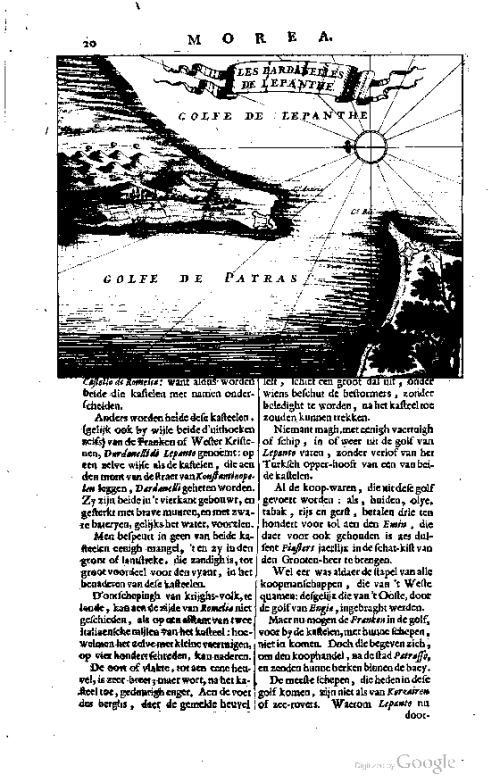
\includegraphics[width=.49\textwidth]{resources/pageImageExample}
		
\includegraphics[width=.49\textwidth]{resources/pageImageExample2}
		\caption{Examples of pages that contain both text and images}
		\label{fig:textImageExamples}
	\end{subfigure}
	\begin{subfigure}[b]{0.49\textwidth}
		
\includegraphics[width=.49\textwidth]{resources/500_0043}
		
\includegraphics[width=.49\textwidth]{resources/500_0010}
		\caption{Examples of pages that consist of text}
		\label{fig:textExamples}
	\end{subfigure}
	\begin{subfigure}[b]{0.49\textwidth}
		
\includegraphics[width=.49\textwidth]{resources/500_0008}
		
\includegraphics[width=.49\textwidth]{resources/500_0077}
		\caption{Examples of pages that consist of images}
		\label{fig:imageExamples}
	\end{subfigure}
	\begin{subfigure}[b]{0.49\textwidth}
		
\includegraphics[width=.49\textwidth]{resources/good_quality}
		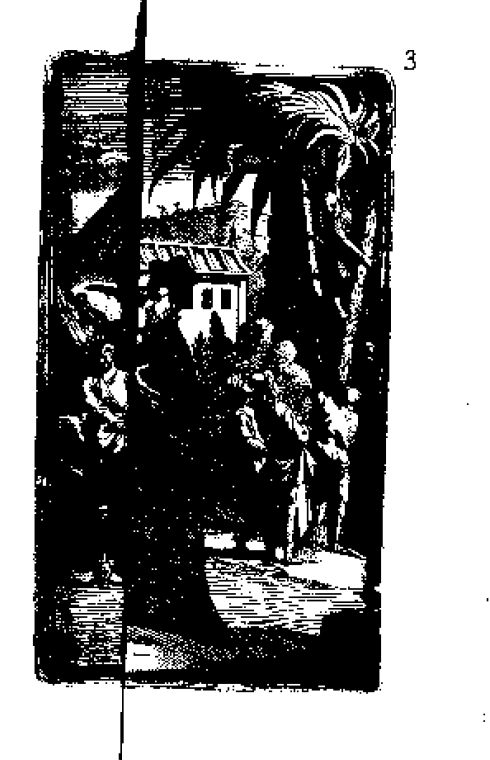
\includegraphics[width=.49\textwidth]{resources/bad_quality}
		\caption{The quality differs per book}
		\label{fig:qualityExamples}
	\end{subfigure}
	\begin{subfigure}[b]{0.49\textwidth}
		
\includegraphics[width=.49\textwidth]{resources/500_0002}
		
\includegraphics[width=.49\textwidth]{resources/500_0004}
		\caption{Some pages contain neither text nor image}
		\label{fig:baggerExamples}
	\end{subfigure}
	\caption{Examples of book pages from the dataset}
%\todo{Fix the new page that occurs before this figure}}
	\label{fig:examples}
\end{figure}
%\restoregeometry
